\documentclass[a4paper,10pt,oneside]{book}
\usepackage[utf8x]{inputenc}

\usepackage{amsfonts}
\usepackage{amsmath} % AMS Math Package
\usepackage{amsthm} % Theorem Formatting
\usepackage{amssymb}	% Math symbols such as \mathbb
% \numberwithin{equation}{chapter}

\usepackage{graphicx} % Allows for eps images
\usepackage[italian]{babel}
\usepackage{setspace}
\singlespacing
\usepackage[strict]{chngpage}
\usepackage{booktabs}
% \usepackage[dvipdf]{graphicx}

\newtheorem{theorem}{Teorema}[section]
\newtheorem{lemma}[theorem]{Lemma}
\newtheorem{proposition}[theorem]{Proposition}
\newtheorem{corollary}[theorem]{Corollary}

%\newenvironment{proof}[1][Dimostrazione]{\begin{trivlist}
%\item[\hskip \labelsep {\bfseries #1}]}{\end{trivlist}}
\newenvironment{definition}[1][Definizione]{\begin{trivlist}
\item[\hskip \labelsep {\bfseries #1}]}{\end{trivlist}}
\newenvironment{example}[1][Example]{\begin{trivlist}
\item[\hskip \labelsep {\bfseries #1}]}{\end{trivlist}}
\newenvironment{remark}[1][Remark]{\begin{trivlist}
\item[\hskip \labelsep {\bfseries #1}]}{\end{trivlist}}

% \newcommand{\qed}{\nobreak \ifvmode \relax \else
%       \ifdim\lastskip<1.5em \hskip-\lastskip
%       \hskip1.5em plus0em minus0.5em \fi \nobreak
%       \vrule height0.75em width0.75em depth0.25em\fi}


\newcommand{\taylor}{\texttt{taylor} }
\newcommand{\cpp}{\texttt{C++}}
\newcommand{\double}{\texttt{double} }
\newcommand{\class}{\texttt{class} }
\newcommand{\template}{\texttt{template} }
\newcommand{\integer}{\texttt{int} }
\newcommand{\size}{\texttt{size }}


% \hyphenation{os-sia}

\usepackage{eso-pic}
\newcommand\BackgroundPic{%
\put(0.,110){%
\parbox[b][1.2\paperheight]{0.5\paperwidth}{%
\vfill
\centering
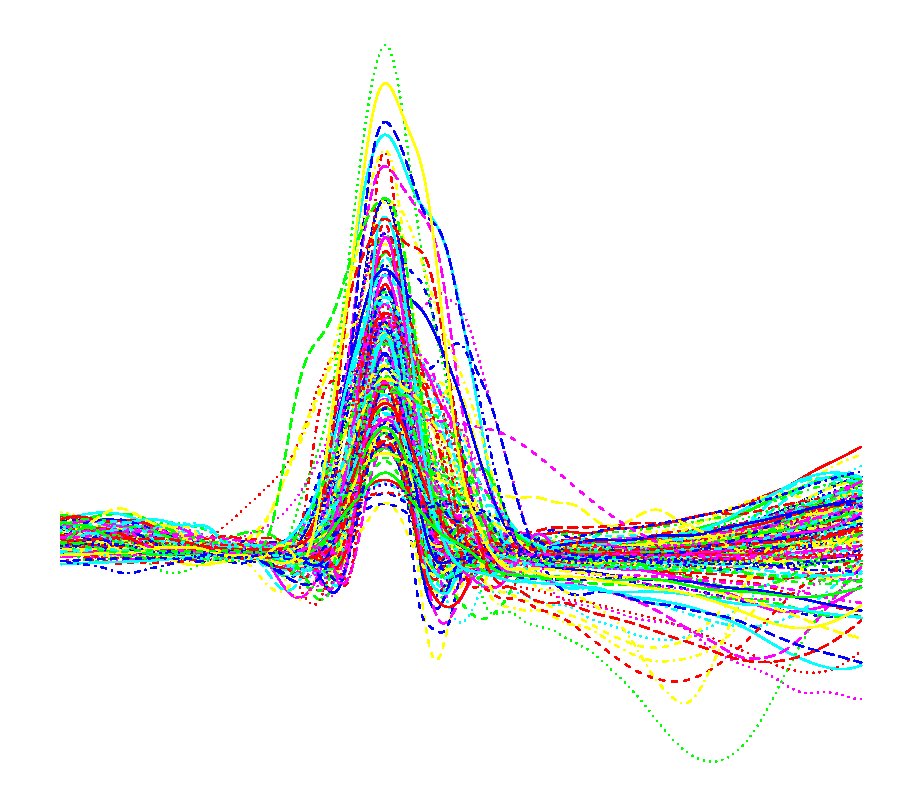
\includegraphics[width=\paperwidth,height=\paperheight,%
keepaspectratio]{img/matplot_trimmed}%
\vfill
}}}

\begin{document}

\begin{titlepage}

\AddToShipoutPicture*{\BackgroundPic}
\voffset = -1 cm

\begin{adjustwidth}{-1 cm}{-1 cm}
\centering
\begin{picture}(400,100)(-250,-50)
\large \textsc{POLITECNICO DI MILANO}
\end{picture}

\vspace{1cm}

% \begin{figure}[h]
%     \begin{adjustwidth}{-1 cm}{-1 cm}\centering
%      
\includegraphics[width = 5 cm]{img/logopoli}
%     \end{adjustwidth}
% \end{figure}

\vspace{1cm}
% \end{spacing}

\vspace*{\stretch{1.5}}

\huge \textsc{Libreria HPCS}\\
  \begin{center}
    \line(1,0){400}
  \end{center}
  \vspace{5mm}
\Large \textsc{ Calcolo di MBD per v.a. funzionali multivariate }\\
  \begin{center}
    \line(1,0){400}
  \end{center}
  \vspace{5mm}
\large {Progetto del corso di Programmazione avanzata per il Calcolo Scientifico}


\vspace*{\stretch{.5}}

\raggedright


 \begin{spacing}{1.2} \Large
 
 \vspace*{\stretch{.5}}
 
 \hspace{8cm} \Large Nicholas Tarabelloni\\
 \hspace{8cm} \Large Matr. n. 782187 \\
 
 \end{spacing}

\vspace*{\stretch{.8}}

\centering
\large \textsc{Anno Accademico 2012-2013}

\end{adjustwidth}

\enlargethispage{3 cm}

\end{titlepage}

\thispagestyle{empty}

\cleardoublepage

\voffset = 0 cm

% \pagenumbering{roman} 

\end{document}